\documentclass{beamer}

\usepackage[utf8]{inputenc}
\usepackage{amsmath}
\usepackage{graphicx}
\usepackage{xcolor}
\usepackage{style}
\usepackage[ddmmyyyy]{datetime}
\usepackage{tabstackengine}
\usepackage{amsmath}
\usepackage{svg}

\title{Kalman Filter}
\subtitle{Grundlagen}
\author{P.~Schön (5121059), C.~Thein (5121017)}
\date{\today}
\renewcommand{\dateseparator}{.}
\newcommand\w[1]{\makebox[2.5em]{$#1$}}

\setbeamertemplate{sections/subsections in toc}[square]
%\setbeamertemplate{sections/subsections in toc}[sections numbered]

\usefonttheme[onlymath]{serif}

\begin{document}

\frame{\titlepage}

\begin{frame}
    \frametitle{Inhaltsverzeichnis}
    \tableofcontents
\end{frame}

\section{Einleitung}

\begin{frame}
    \frametitle{What is the Kalman Filter?}
    The Kalman filter is a mathematical method for iteratively estimating parameters to describe 
    system states.

    In this process, a prediction about a parameter value is repeatedly made, combined with the 
    error-prone measurement, and then used again to make a new prediction.
\end{frame}

\section{Vereinfachte Erklärung}

\begin{frame}
    \frametitle{Process of Kalman Filters}

    \textbf{Prediction}

    1. State prediction: \( \hat{x}_{k} = A\hat{x}_{k-1}+Bu_{k-1} \)

    2. Covariance prediction: \( P_{k}=AP_{k-1}A^{T}+Q \)

    \textbf{Correction}

    3. Kalman Gain Prediction: \( K_{k}=P_{k}H^{T}(HP_{k}H^T+R)^{-1} \)

    4. State Update: \( \hat{x}_{k}=\hat{x}_{k}+K_{k}(z_{k}-H\hat{x}_{k}) \)

    5. Covariance Update: \( P_{k}=(I-K_{k}H)P_{k} \)
\end{frame}


\begin{frame}
    \frametitle{Kalman explained}
    \begin{figure}
        \centering
        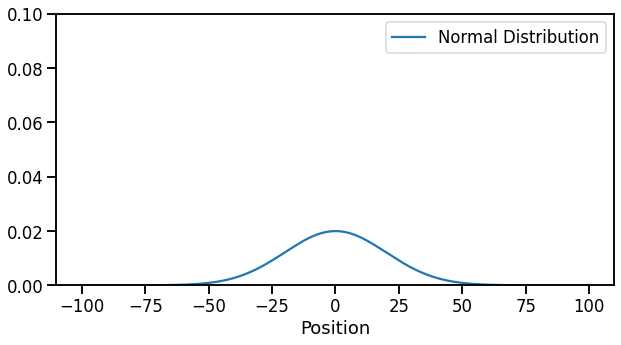
\includegraphics[width=0.7\textwidth]{images/01_normal_distribution.png}
        \caption{Start Postion at \(t_0\)}
    \end{figure}
\end{frame}

\begin{frame}
    \frametitle{Kalman explained}
    \begin{figure}
        \centering
        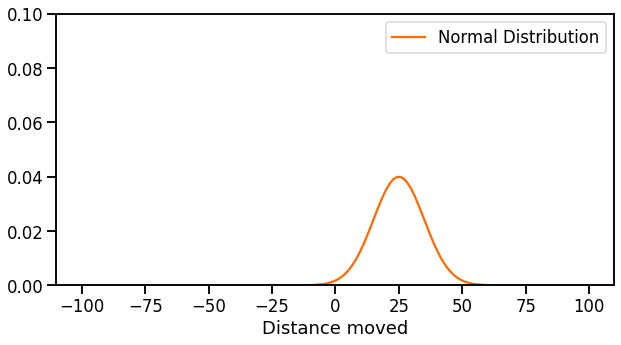
\includegraphics[width=0.9\textwidth]{images/02_normal_distribution_after_move.png}
        \caption{Calculated Postion at \(t_1\)}
    \end{figure}
\end{frame}

\begin{frame}
    \frametitle{Kalman explained}
    \begin{figure}
        \centering
        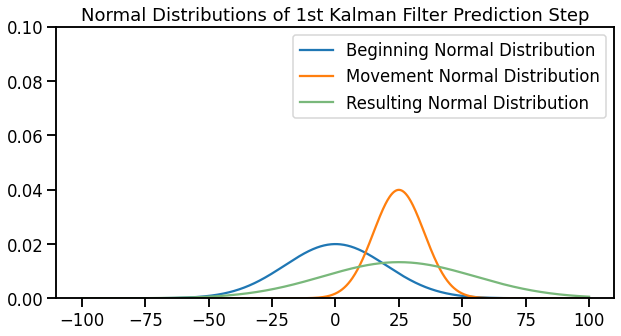
\includegraphics[width=0.9\textwidth]{images/03_first_prediction.png}
        \caption{Predicted Postion at \(t_1\)}
    \end{figure}
\end{frame}

\begin{frame}
    \frametitle{Kalman explained}
    \begin{figure}
        \centering
        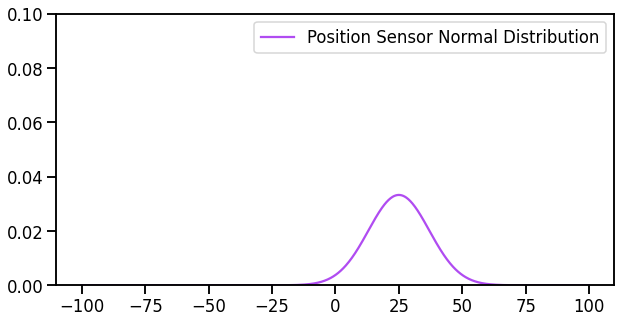
\includegraphics[width=0.9\textwidth]{images/04_measurement.png}
        \caption{Messured Sensor Data of Postion at \(t_1\)}
    \end{figure}
\end{frame}

\begin{frame}
    \frametitle{Kalman explained}
    \begin{figure}
        \centering
        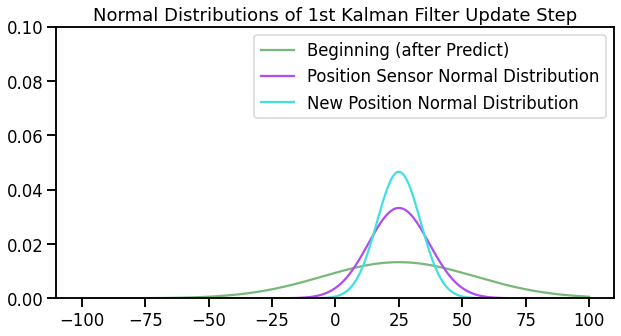
\includegraphics[width=0.9\textwidth]{images/05_correction.png}
        \caption{Correction of the Kalman Gain after Messurement at \(t_1\)}
    \end{figure}
\end{frame}

\begin{frame}
    \frametitle{Takeaways}
    \begin{itemize}
        \item The precision sinks with the prediction
        \item The precision grows with the correction
    \end{itemize}
    
\end{frame}

\section{Joystick example}

\begin{frame}
    \frametitle{State Representation}
    % //TODO: Make x's differentiabable
    We define the state vector \(x\) to include the position and velocity of the mouse in both x and y directions
   
    \begin{equation*}
        x = \begin{bmatrix}
            x      \\
            y      \\
            v_{x}  \\
            v_{y}  \\
        \end{bmatrix}
    \end{equation*}

    where:
    \begin{itemize}
        \item \(x\) is the position on the x-axis
        \item \(y\) is the postion on the y-axis
        \item \(v_{x}\) is the velocity in the x-direction
        \item \(v_{y}\) is the velocity in the y-direction

    \end{itemize}
\end{frame}

\begin{frame}
    \frametitle{Formulate the Transtition Model}
    The state transition model describes how the state evolves from one time step to the next. 
    If we assume a constant velocity model, the state transition can be expressed as:
    \begin{equation*}
        x_{k+1}=Ax_{k}+w_{k}
    \end{equation*}
    where \(w_{k}\) represents the proces noise, assumed to be Gaussian with zero mean and covariance \(Q\).
\end{frame}

\begin{frame}
    \frametitle{Create the Transition Matrix}
    The transition matrix A for a constant velocity Model is: 
    
    \begin{equation*}
        A = \begin{bmatrix}
            1 & 0 & \Delta t & 0        \\
            0 & 1 & 0        & \Delta t \\
            0 & 0 & 1        & 0        \\
            0 & 0 & 0        & 1        \\ 
        \end{bmatrix}
    \end{equation*}

    \(\Delta t\) is the time intervall between mesurements.
\end{frame}

\begin{frame}
    \frametitle{Observation Model}
    The observation model realtes the state to the measurements:
    \begin{equation*}
        z_{k}=Hx_{k}+v_{k}
    \end{equation*}
    where \(v_{k}\) represents the measurement noise, assumed to be Gaussian with zero mean and
    covariance \(R\).

    The observation matrix \(H\) for direct measurement of position is:
    
    \begin{equation*}
        H = \begin{bmatrix}
            1 & 0 & 0 & 0 \\
            0 & 1 & 0 & 0 \\
        \end{bmatrix}
    \end{equation*}

\end{frame}

\begin{frame}
    \frametitle{Prediction Step}
    
    The prediction step estimates the next state and its uncertainty:

    \begin{itemize}
        \item Predict the state:
        \begin{equation}
            x_{k+1}=Ax_{k} 
        \end{equation}

        \item Predict the error coavriance:
        \begin{equation}
            P_{k+1}=AP_{k}A^{T}+Q
        \end{equation}
    \end{itemize}
\end{frame}

\begin{frame}
    \frametitle{Correction Step}
    The correction step updates the state estimate with the new measurement:
    \begin{itemize}
        \item Compute the Kalman gain:
            \begin{equation}
                K_{k} = P_{k}H^{T}(HP_{k}H^{T}+R)^{-1}
            \end{equation}
        \item Update the state estimate:
            \begin{equation}
                x_{k} = x_{k}+K_{k}(z_{k}-Hx_{k})
            \end{equation}
        \item Update the error covariance:
            \begin{equation}
                P_{k} = (I-K_{k}H)P_{k}
            \end{equation}
    \end{itemize}
\end{frame}

\begin{frame}
    \frametitle{Kalman Filter}
    \begin{figure}
        \centering
        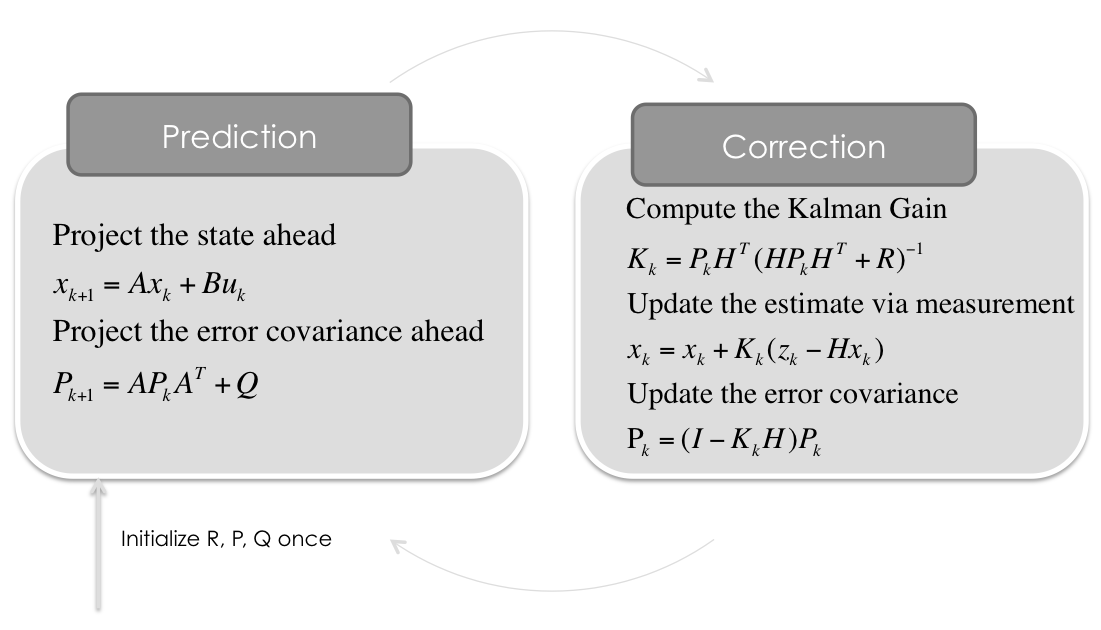
\includegraphics[width=0.95\textwidth]{images/06_kalman_diagram.png}
        \caption{Iterative Nature of the Kalman filter}
    \end{figure}
\end{frame}

\begin{frame}
    \frametitle{Cheat Sheet - Math Symbols}
    \begin{table}[h]
        \centering
        \begin{tabular}{|l|p{8cm}|}
        \hline
        \textbf{Symbol} & \textbf{Meaning} \\ \hline
        \(k\)          & Interval / iteration of the Kalman filter\\ \hline
        \(z_k\)       & Measurement from the sensor  \\ \hline
        \(x_k\)       & Value of the current estimation \\ \hline
        \(x_{k-1}\)   & Value of the previous estimation \\ \hline
        \(P_k\)       & Value of the current error covariance \\ \hline
        \(P_{k-1}\)   & Value of the previous error covariance \\ \hline
        % //TODO: Translate to english
        \(R\)          & Variance of the measurements \\ \hline
        \(Q\)          & Process noise covariance \\ \hline
        \(A\)          & Transition Matrix \\ \hline
        \(H\)          & Observation Matrix \\ \hline
        \(Bu_{k-1}\) & Control signal \\ \hline
        \end{tabular}
        \end{table}
\end{frame}

\section{Summary}

\begin{frame}
    \frametitle{Summary}
    KALMA KALMA !
\end{frame}

\end{document}
\ProvidesPackage{beamerthemesss}
\mode<presentation>
\usepackage{xcolor}
\usepackage{tikz}
\RequirePackage{enumitem} 


\definecolor{orange_100}{RGB}{255, 107, 0} 	% orange_100
\definecolor{orange_80}{RGB}{255, 137, 51} 	% orange_80
\definecolor{black_100}{RGB}{0, 0, 0} 		% black_100
\definecolor{black_80}{RGB}{50, 50, 50} 		% black_80
\definecolor{black_60}{RGB}{100, 100, 100} 	% black_60
\definecolor{white}{RGB}{255, 255, 255} 		% white


% Define a command to set the foreground color of lists
\newcommand{\setlistcolor}[1]{
    \setlist[enumerate]{label=\textcolor{#1}{\textbullet}}
    \setlist[itemize]{label=\textcolor{#1}{\textbullet}}
}
\setlistcolor{orange_80}

% Schriftarten einstellen
\setbeamerfont{title}{size=\huge,series=\bfseries}
\setbeamerfont{subtitle}{size=\small,series=\bfseries}
\setbeamerfont{frametitle}{size=\large,series=\bfseries}
\setbeamerfont{normal text}{size=\small}

% Farben anwenden
\setbeamercolor{title}{fg=orange_100}
\setbeamercolor{subtitle}{fg=black_60}
\setbeamercolor{frametitle}{fg=orange_100}
\setbeamercolor{section in toc}{fg=black_80}
\setbeamercolor{normal text}{fg=black_80}
\renewcommand{\figurename}{\textcolor{orange_100}{Fig.}}

% Layout anpassen
\setbeamertemplate{navigation symbols}{}

% Customize header and footer with dotted lines made of circles
\setbeamertemplate{headline}{
    \begin{tikzpicture}[remember picture,overlay]
    	\ifnum\theframenumber=1
        \node[anchor=north east, inner sep=0pt, yshift=-0.5mm, xshift=-2mm] at (current page.north east) {
            
\includegraphics[height=4.8mm]{logo.png}
        };
        \fi
        \draw[thick, dash pattern=on 0pt off 2\pgflinewidth, line cap=round, color=orange_100]
              ([yshift=-7.5mm]current page.north west) -- 
              ([yshift=-7.5mm]current page.north east);
    \end{tikzpicture}
}

\setbeamertemplate{footline}{
    \begin{tikzpicture}[remember picture,overlay]
        \ifnum\theframenumber>1
        	\draw[thick, dash pattern=on 0pt off 2\pgflinewidth, line cap=round, color=orange_100] 
              ([yshift=8mm]current page.south west) -- 
              ([yshift=8mm]current page.south east);
                      \node[anchor=east, inner sep=0pt, yshift=2.5mm, xshift=-5mm] at (current page.south east) {
        					\color{black_60}
        					\insertframenumber/
        					\inserttotalframenumber
        	};
        	\node[anchor=west, inner sep=0pt, yshift=3.5mm, xshift=-2mm] at (current page.south west) {
        		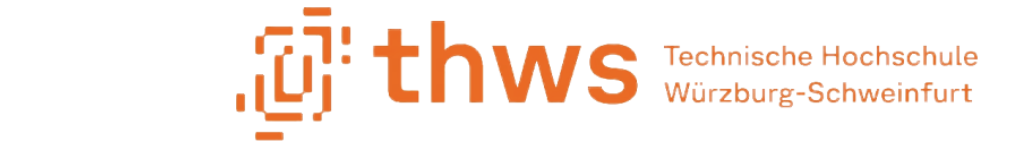
\includegraphics[height=7.8mm]{watermark.png}
        	};
        \fi
        \ifnum\theframenumber=1
        	\node[anchor=west, inner sep=0pt, yshift=6mm, xshift=-4mm] at (current page.south west) {
        		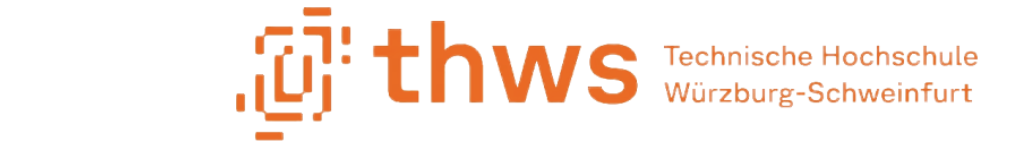
\includegraphics[height=9.8mm]{watermark.png}
        	};
        \fi

    \end{tikzpicture}
}

% Abschnittsüberschriften
\setbeamercolor{section in head/foot}{bg=orange_100,fg=white}
\setbeamerfont{section in head/foot}{series=\bfseries}
\setbeamertemplate{section in head/foot shaded}{\color{orange_100!50}}

\setbeamertemplate{frametitle}{
    \begin{tikzpicture}[remember picture,overlay]
        \node[
        	anchor=base west, 
        	fill=white, 
        	yshift=-3.9mm, 
        	xshift=-2mm
        ] {\bfseries\insertframetitle};
    \end{tikzpicture}
}


\endinput

